\section{List of hardware} \label{app:hardwareused}

The hardware listed below is a comprehensive minimal list that is required for the system.
Additionally, light sources should be used as necessary.

\begin{itemize}
	\item 9 x Canon EOS 700D DSLR camera body
	\item 9 x Canon EF 50mm f/1.8 II lens
	\item 9 x Canon ACK-E8 Power adapter (one for each)
	\item 9 x Transcend SDHC class 10 UHS-I 16GB memory card
	\item 9 x Manfrotto 494 ball head
	\item 9 x Manfrotto 035 Super Clamp, with Manfrotto 036-38 studs
	\item 3 x D-link DUB-H4 USB hub
	\item 4 x Millenium LST-310, a sturdy three-legged lighting stand with a pole that can be extended several meters high.
	\item Custom built remote trigger board using ST Nucleo-F401RE, see Section \ref{app:remotetrigger}
	\item Canon RC-6 wireless remote control for testing
	\item Auxiliary extension cords
	\item 2 x bags for the stands
	\item 2 x hard equipment cases with cut holes for all smaller parts of the rig
\end{itemize}

%\clearpage

\section{Remote trigger} \label{app:remotetrigger}

The designed remote trigger consists of a Nucleo-F401RE microcontroller platform by ST microelectronics \cite{stnucleo}, and supporting hardware for connecting the cameras.
The microcontroller was programmed using the Mbed library for the particular microcontroller. \cite{mbednucleo}
Each camera connects to the trigger via a 2,5mm stereo plug, as the cameras have a standard 2,5mm jack for remote trigger.
To secure the cameras from each other, the remote wires are connected with opto-isolators (TLP621-2).

The ground signals of the isolators in the built circuit are connected together by mistake, so the cameras are not completely isolated - only their signal wires are.
However, common grounding is generally not an issue.
Furthermore, the USB connections of all cameras also connect to each other and to the trigger box via the computer they are connected to, which cannot be easily circumvented.
The diagrams depicted in this section show the fixed versions; the older ones used in the production device can be found in the git repository history at \url {http://github.com/sooda/thesis} if necessary.
The repository contains the project files for the Cadsoft EAGLE pcb design software \cite{eaglepcb}; the diagrams for schematic and PCB layout are given here for illustration only.

\subsection{Schematic} \label{app:fullschematic}

\simplefig{p}{%
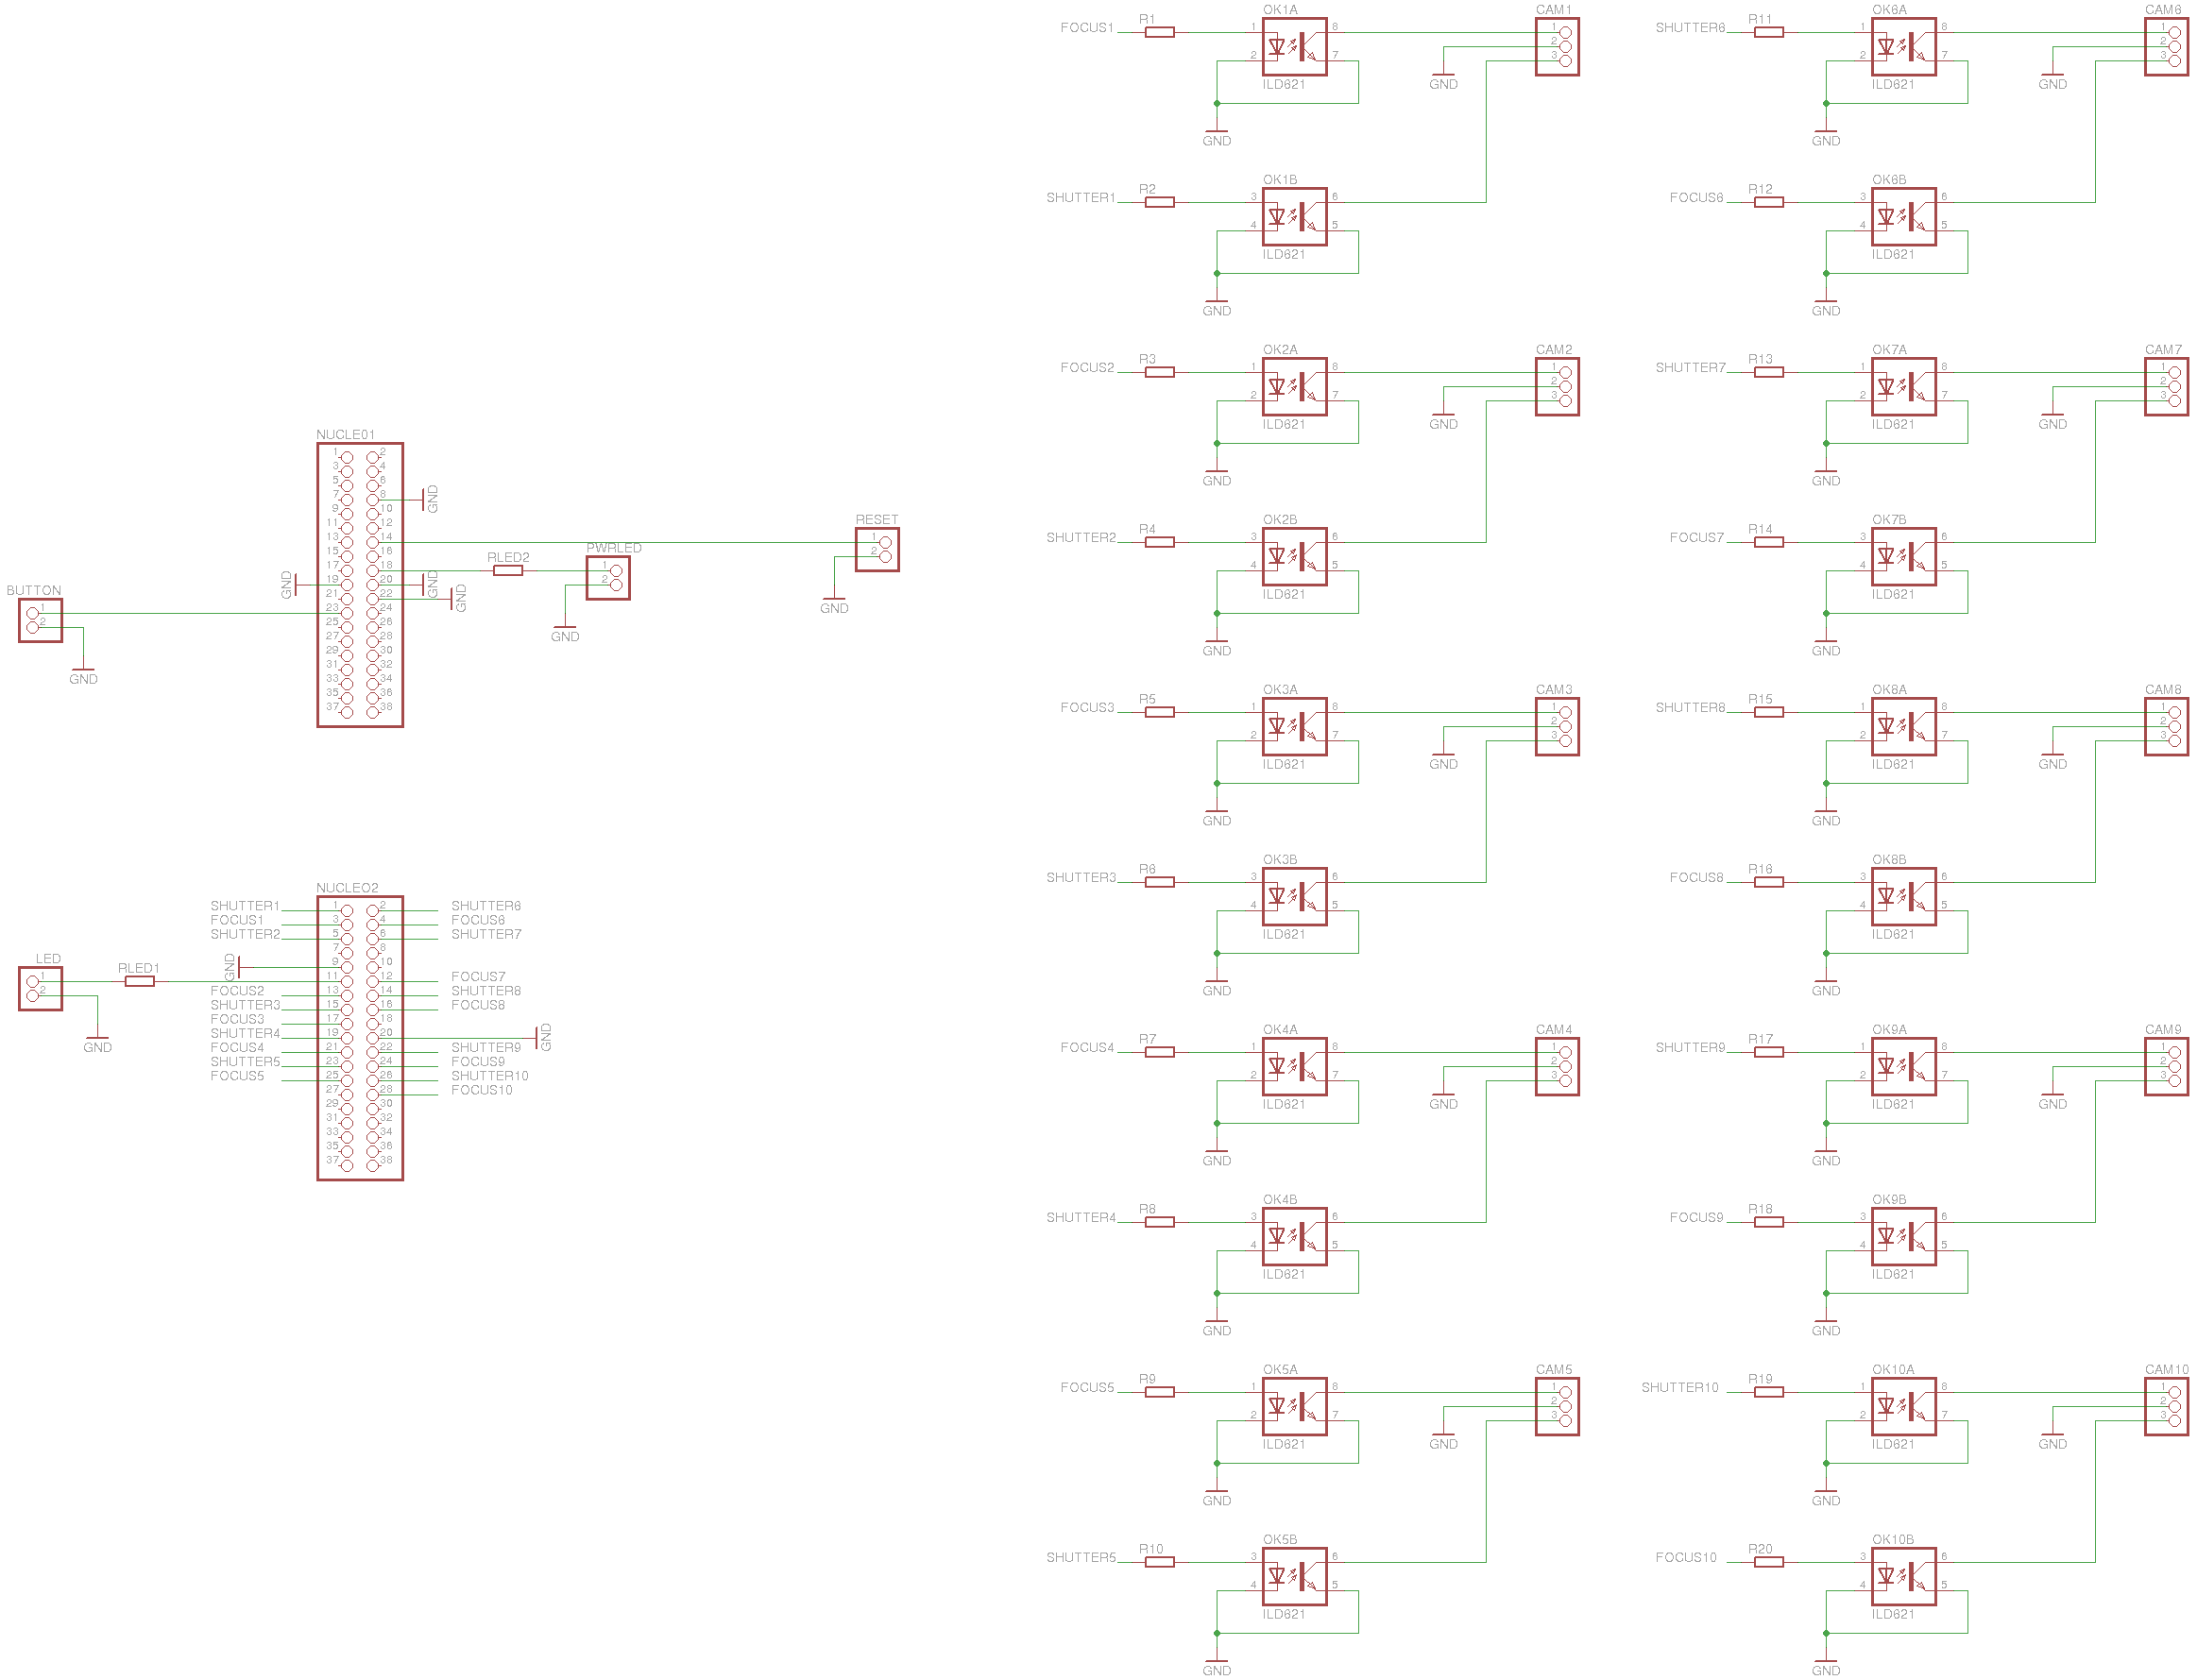
\includegraphics[height=\textwidth, angle=90]{triggerboard-sch}
}{fig:triggerboard-sch-big}
{Remote trigger schematic}

See Figure \ref{fig:triggerboard-sch-big} for a complete schematic.
The two pin headers are those of the Nucleo board, and the order of the opto-isolators and connectors matches with the physical order of the connectors on the PCB.
Additionally, the LEDs and buttons were routed to the side of the board to be accessible when installed in the enclosure.

\subsection{Printed circuit board layout}

\simplefig{p}{%
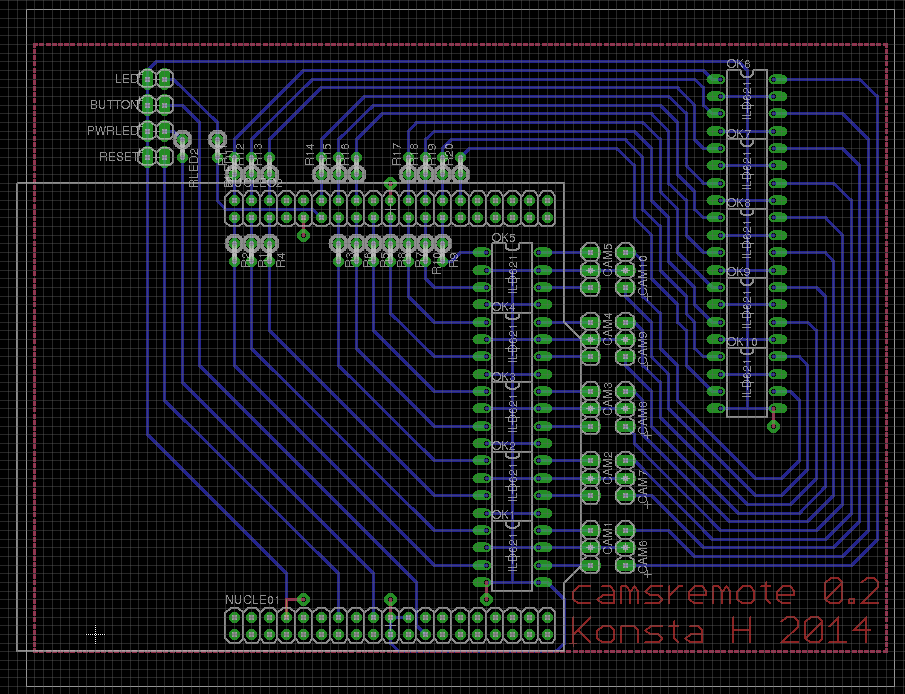
\includegraphics[height=\textwidth, angle=90]{triggerboard}
}{fig:triggerboard-brd-big}
{Remote trigger circuit board (PCB) layout}

The circuit board dimensions are 5 by 3.9 inches (approximately 127 by 99 mm) designed to fit in the given enclosure.
All electrical connections can be realized with just one layer;
another layer was used as a ground plane, but the ground signals are routed also along with the signals.
The circuit is also simple enough to implement on e.g. a prototyping board with jumper wires.
Figure \ref{fig:triggerboard-brd-big} shows the board layout without a ground plane drawn.

\subsection{Finished device}

\simplefig{p}{%
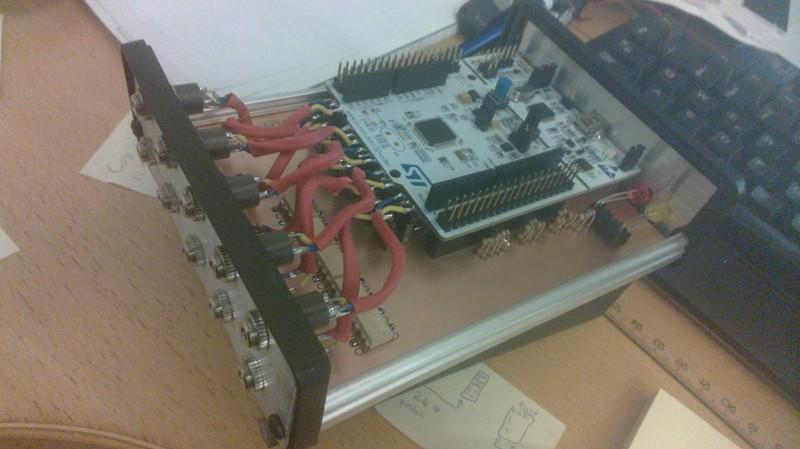
\includegraphics[height=\textwidth, angle=90]{camsremote}
}{fig:camsremote-full}
{Components installed to the board and fitted in the enclosure}

The PCB was built with a milling machine produced by LPKF Laser \& Electronics AG.
A recycled enclosure was used with custom drilled end caps for the 2,5 mm jacks for the camera connections in one end, and Nucleo board's micro-USB, LEDs and buttons on other end.
Of the two buttons, the red one is the user button, and black one is the reset button.
The red LED shows that the power is on, and the yellow LED is on when the focus command has been received.

The device is shown in Figure \ref{fig:camsremote-full}, and Figure \ref{fig:camsremote-full} shows the same with the case opened, exposing the circuit board, soldered parts and the connectors mounted on the end.

%Much of the physical space is taken by the microcontroller board and the bulky through-hole mounted opto-isolators.
%The size of the trigger box could be reduced to approximately half of its size by using surface mount opto-isolators and designing the microcontroller itself on the same circuit board, removing the large pin headers.
%This was not a high priority, though, as the whole trigger device is already small compared to the whole system.

%\clearpage

\subsection{Parts list}

\begin{itemize}
	\item ST Microelectronics Nucleo-F401RE microcontroller platform
	\item Mini USB cable
	\item 10 x stereo 2,5 mm jack
	\item 10 x stereo 2,5 mm plug-plug 3 meter cable
	\item 10 x TLP621-2 opto-isolator; interchangeable with any with identical pinout
	\item 20 x 220 ohm resistor
	\item With an enclosure, two LEDs with current limiting resistors and two pushbuttons should be used
\end{itemize}
